\documentclass[11pt,a4paper]{beamer}

\usetheme[progressbar=frametitle]{metropolis}
\setbeamertemplate{frame numbering}[fraction]
\useoutertheme{metropolis}
\useinnertheme{metropolis}
\usefonttheme{metropolis}
\usecolortheme{spruce}
\setbeamercolor{background canvas}{bg=white}
\definecolor{mygreen}{rgb}{.125,.5,.25}
\usecolortheme[named=mygreen]{structure}

\usepackage{graphicx}

\usepackage{listings}
\lstset{numbers=left, numberstyle=\tiny, numbersep=5pt}
\lstset{language=R}

\logo{
\includegraphics[width=1.5cm]{553400.jpg}}
\author{Bradley Mackay, Clemens Ehlich}
\title[Short Title]{R-Packages}
\subtitle{Statistics, Visualization and more using R}
\institute{NAWI PLUS}
\date{}



\begin{document}
	%\metroset{block=fill}
	
%Titelblatt

	\begin{frame}
	
		\titlepage
	\end{frame}

%Folie_2

	\begin{frame}[t]{Syllabus}
	
		\begin{enumerate}
			\item One
			\begin{enumerate}
				\item Two
				\item Three
				\item Four
			\end{enumerate}
			\item Five
			\item Six
		\end{enumerate}
		
	\end{frame}



\begin{frame}[t]{1. Introduction}
	

\begin{figure}
	\centering
	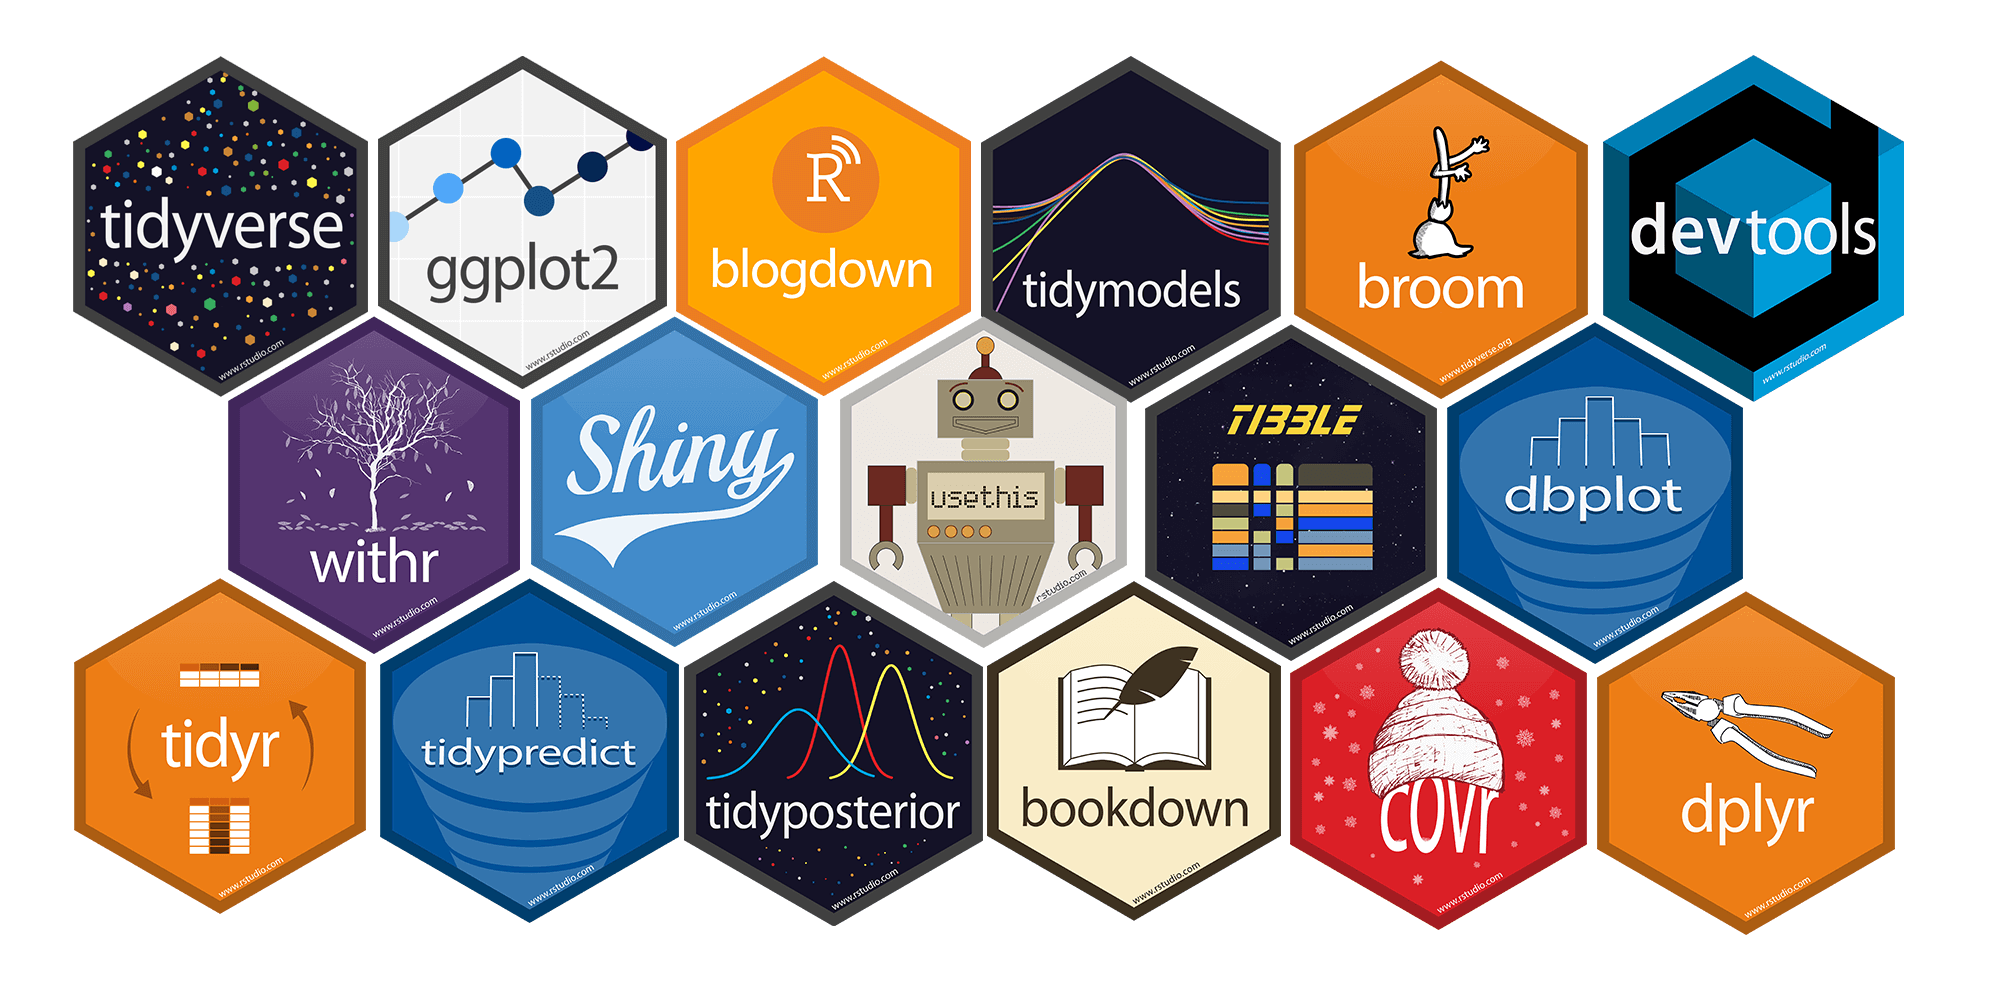
\includegraphics[width=0.9\linewidth]{packages}
%	\caption{}
	\label{fig:packages}
\end{figure}

	
\end{frame}










%Folie_3
		\begin{frame}[t]{1.1 What's a package?}
				
		\begin{itemize}
			\item R packages are collections of functions and data sets  
			\item they extend the basic functionalities or add new ones
			\item mostly developed by the community itself 
			
			
		\end{itemize}
		
	\end{frame}
	
%Folie_4	
	
	\begin{frame}[t]{1.2 Why Packages?}
		
	
		\begin{itemize}
			\item easy method for sharing your code with others 
			\item recurring tasks - no need to reinvent the wheel
			\begin{itemize}
				\item[--] to load data
				\item[--] to manipulate data
				\item[--] to visualize data
				\item[--] etc. (more than 19.000 packages exist)
			\end{itemize}
			\item packages form interfaces to:
			\begin{itemize}
				\item[--] other software and their file formats (foreign, caffe, RQGIS, ...)
				\item[--] databases (RODBC, RPostgreSQL, ...)
				\item[--] other programming languages (Rcpp, RPython, ...)
				\item[--] webservices (Rfacebook, RGoogleAnalytics, ...)
			\end{itemize}
		\end{itemize}
	
	\end{frame}




%Folie_5

\begin{frame}[t]{1.3 Where can you find packages?}
	
		
	\begin{itemize}
		\item CRAN -  The Comprehensive R Archive Network 
		
			\begin{itemize}
				\item[] https://cran.r-project.org 
			\end{itemize}
		
		\item BioConductor
		
			\begin{itemize}
				\item[] http://bioconductor.org/
			\end{itemize}
	
		\item GitHub
	
			\begin{itemize}
				\item[] https://github.com/
			\end{itemize}
		
		\item The most comfortable way is to use \textit{RDocumentation}, because you can search more than 19.000 CRAN, Bioconductor and GitHub packages at onces.
	
			\begin{itemize}
				\item[] https://www.rdocumentation.org/ also available as a package
			\end{itemize}
			
	\end{itemize}
	
\end{frame}




%%Folie_6


\begin{frame}[t]{1.4 Install, Deinstall, Update}
	

		\begin{block}{Install:}
			\begin{itemize}
				\item[] install.packages("xyz") 
				\item[]install.packages(c("xyz", "123"))
			\end{itemize}
		\end{block}
	

		\begin{block}{Deintall:}
			\begin{itemize}		
				\item[] remove.packages("xyz")
			\end{itemize}
		\end{block}


		\begin{block}{Update:}
			\begin{itemize}
				\item[] old.packages() $ \rightarrow $ check what packages need an update
				\item[] update.packages() $ \rightarrow $ update packages
			\end{itemize}
		\end{block}
\end{frame}




%%Folie_7


\begin{frame}[t]{1.4.1 Installing packages via devtools}
	
	\begin{itemize}
		\item one big problem: each repository has its own way to install a package from them
		\item to simplify this process you can use the package "devtools"
		\item but you might also need to install: 
		\begin{itemize}
			\item[--]"Rtools" for Windows
			\item[--]"Xcode" for Mac 
			\item[--]"r-devel and r-devel" for Linux
		\end{itemize}
			
	\end{itemize}

\end{frame}


%%Folie_7


\begin{frame}[t]{1.4.2 Installing packages via devtools}
After devtools is installed, you will be able to use the utility functions to install another packages. Some options are:
\begin{itemize}
	\item[--]install\_bioc() from Bioconductor
	\item[--]install\_cran() from CRAN
	\item[--]install\_github() from GitHub
	\item[--]install\_local() from a local file
	\item[--]install\_url() from a URL
\end{itemize}

Example: 
devtools::install\_github("hadley/babynames")


\end{frame}






\begin{frame}[t]{2. Making our own package}
	

	
	\begin{figure}
		\centering
		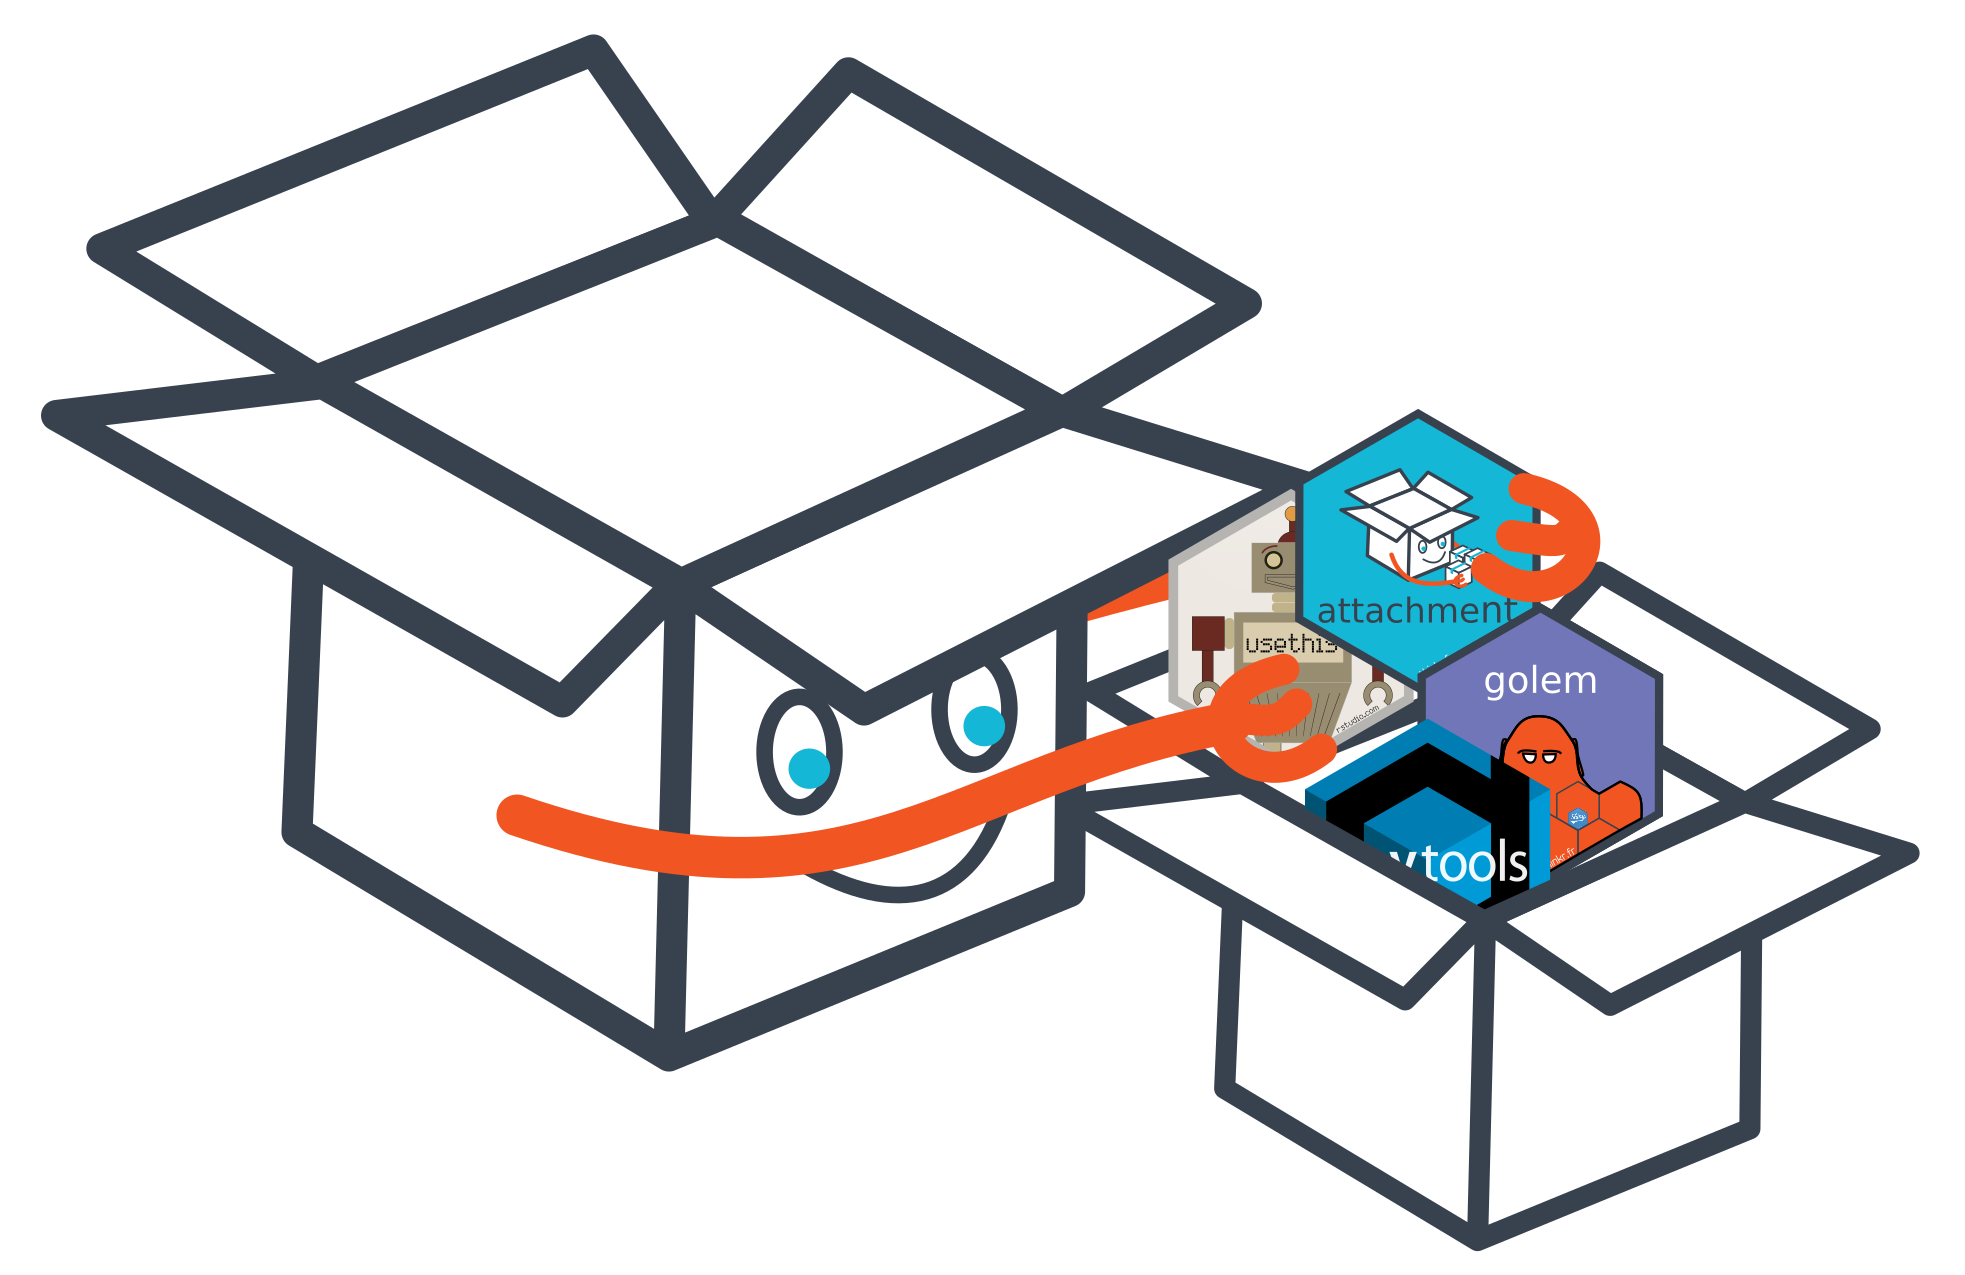
\includegraphics[width=0.9\linewidth]{user}
		
		%\caption{}
		\label{fig:packages}
	\end{figure}
	
	
\end{frame}





\begin{frame}[t]{2.1 Making our own package}
	
	\begin{itemize}
		\item Hadley Wickham - Chief Scientist at RStudio, Adjunct Professor of Statistics at the University of Auckland, Stanford University, and Rice University
		\item Free to read Book "R Packages": \textbf{http://r-pkgs.had.co.nz/}
		\item https://cran.r-project.org/doc/manuals/r-release/R-exts.html
			
	\end{itemize}

	\begin{figure}
	\centering
	
\includegraphics[width=0.3\linewidth]{hadley}
	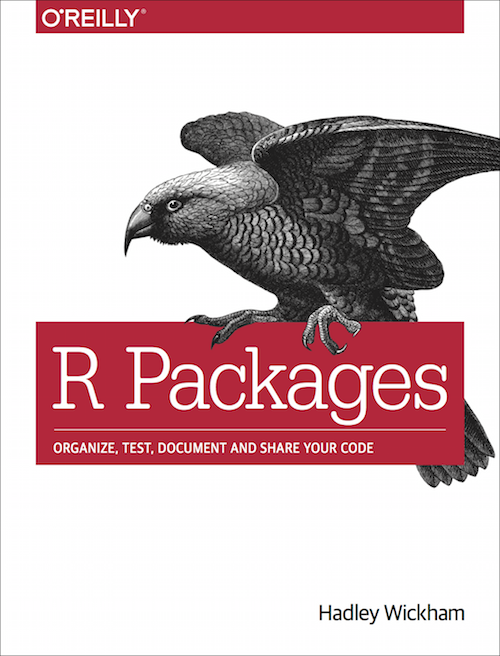
\includegraphics[width=0.3\linewidth]{cover}
	%\caption{}
	\label{fig:packages}
	\end{figure}

	
\end{frame}










%%Folie_7

\begin{frame}[t]{2.1.0 Structure of a package?}
	
	
	
	\begin{itemize}
		\item 
		\item a package is a directory of files which extend 
	
	
	\end{itemize}
	
\end{frame}

\begin{frame}[t]{2.1 Structure of a package?}
	
	
	\begin{figure}
		\centering
		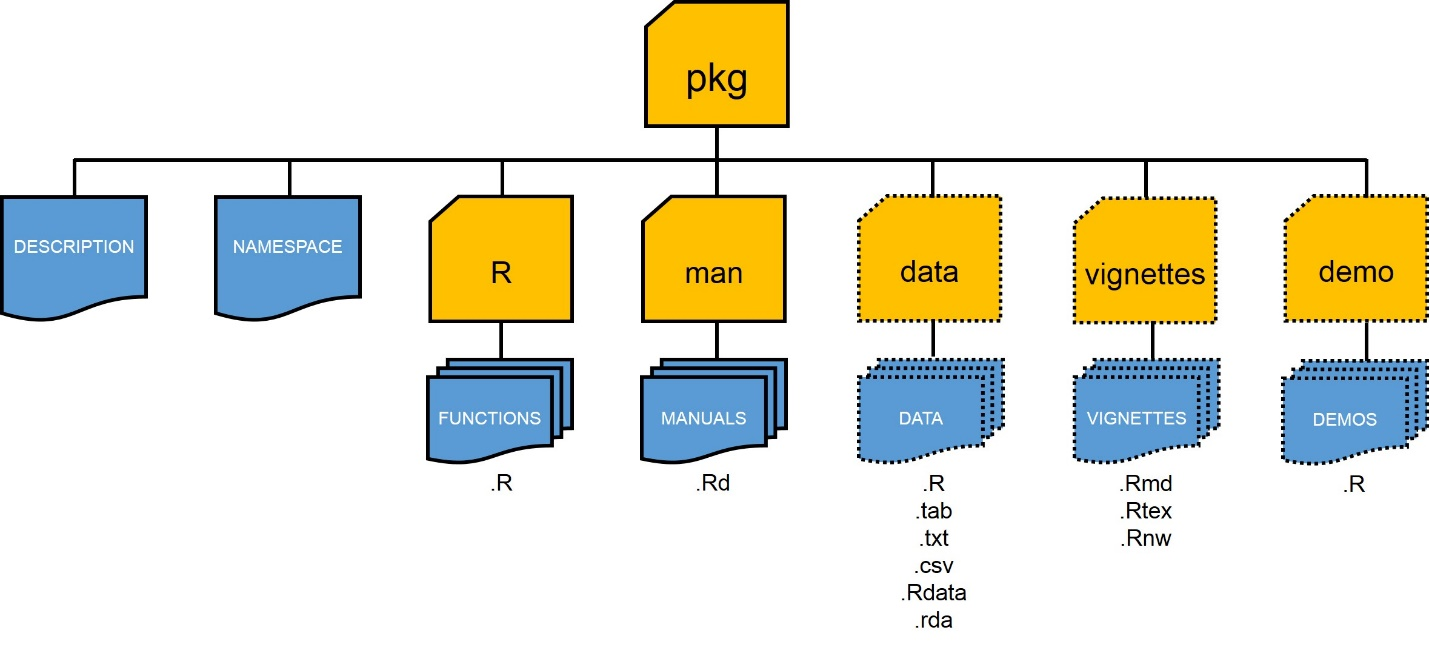
\includegraphics[width=0.9\linewidth]{stott}
		%	\caption{}
		\label{fig:packages}
	\end{figure}
	
	
\end{frame}

\begin{frame}[t]{2.1.1 Description File}
	
	
	\begin{figure}
		\centering
		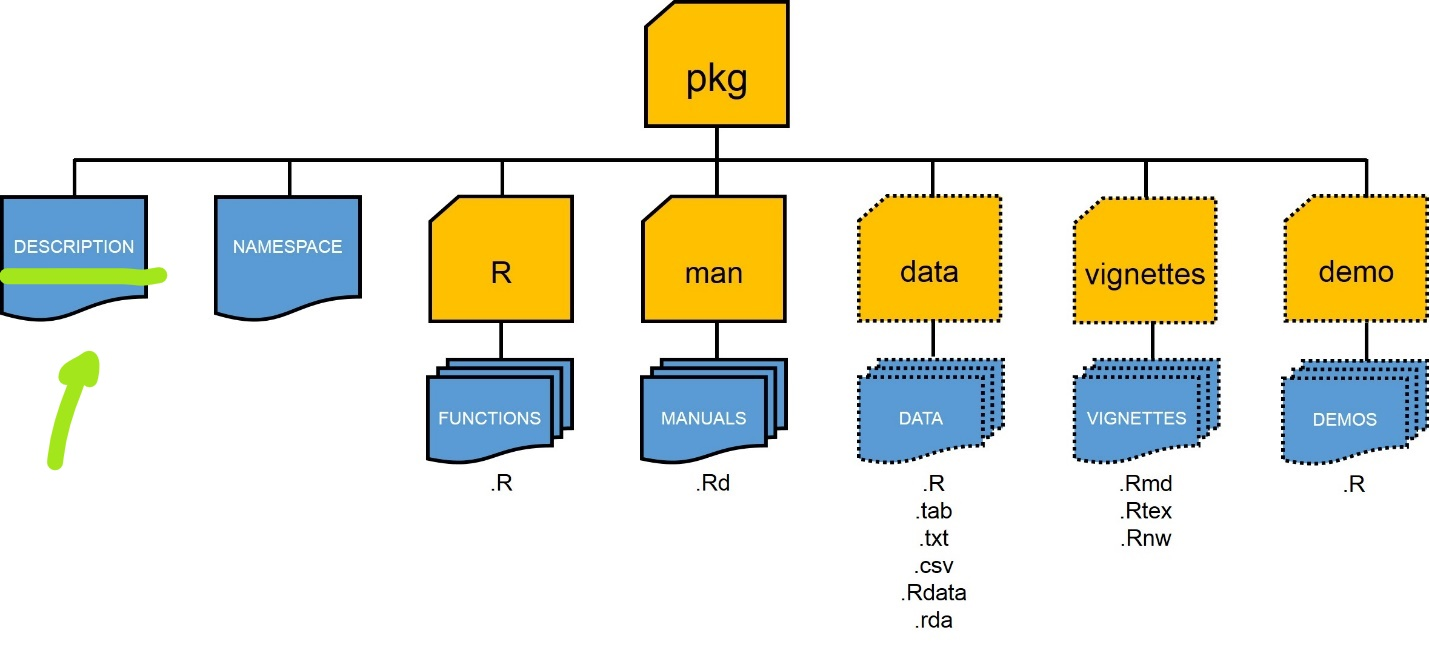
\includegraphics[width=0.9\linewidth]{Desc}
		%	\caption{}
		\label{fig:packages}
	\end{figure}
	
	
\end{frame}

\begin{frame}[t]{2.1.1 Description File}
	
	\begin{itemize}
		\item Title	
		\item Description
		\item Dependencies
		\begin{itemize}
			\item  list of necessary packages (and also package versions)
			\item "LinkingTo" a Package - if you want to use c or c++ code from another package
		\end{itemize}
		\item Author	
		\item License (MIT, GPL-2, ...)
		
	\end{itemize}
	
\end{frame}




\begin{frame}[t]{2.1.2 Namespace}
	
	
	\begin{figure}
		\centering
		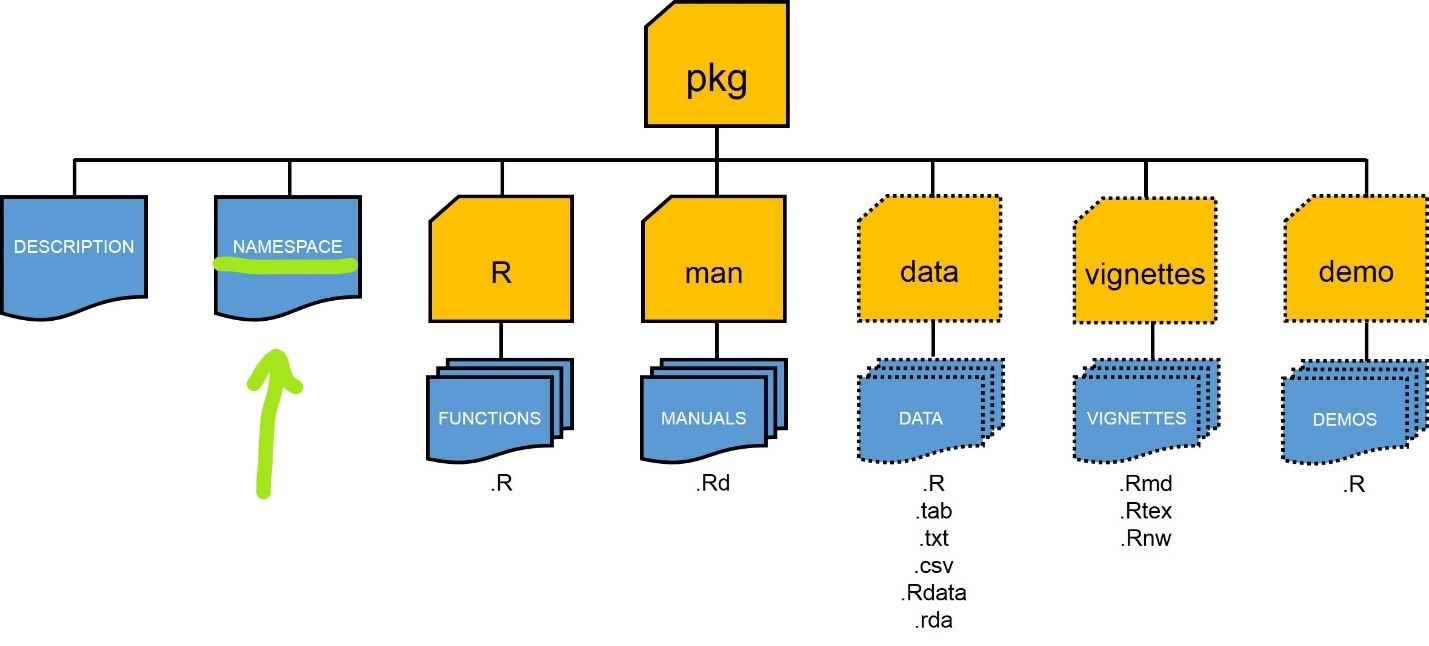
\includegraphics[width=0.9\linewidth]{Names}
		%	\caption{}
		\label{fig:packages}
	\end{figure}
	
	
\end{frame}




\begin{frame}[t]{2.1.2 Namespace}
	
	\begin{itemize}
		\item With NAMESPACE you define  the way in which your package interacts with other packages. For Example, to:
		\begin{itemize}
			\item ensure that other	packages won’t	interfere	with the code you include 
			\item	your code	won’t	interfere	with	other	packages 	
			\item and	that	your	package	works	regardless	of	the
			environment	in	which	it’s	run
		\end{itemize}
		
		
		\item Practical example: You are using two packages with "::	operator" and both have the summarize() function. Then it does matter in which order the packages are loaded in your code. 
		
	\end{itemize}
	
\end{frame}






\begin{frame}[t]{2.1.3 R-Functions}
	
	
	\begin{figure}
		\centering
		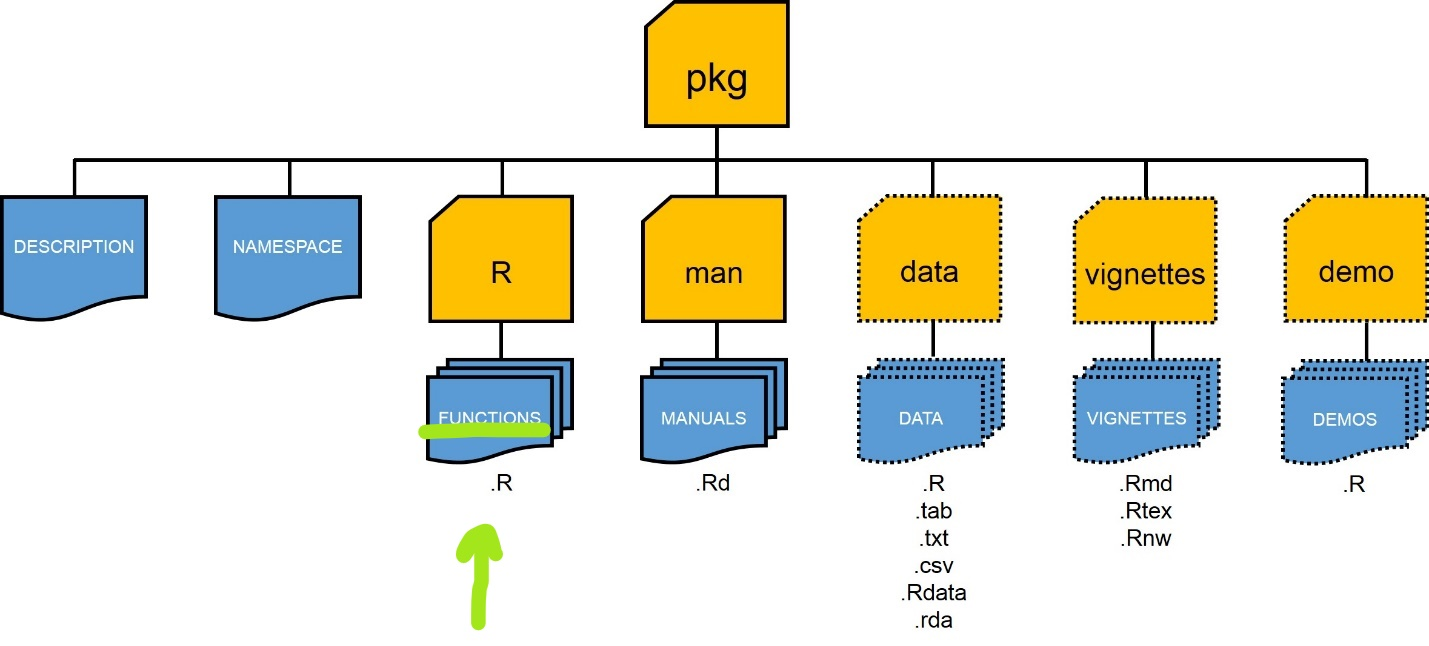
\includegraphics[width=0.9\linewidth]{Rfunc}
		%	\caption{}
		\label{fig:packages}
	\end{figure}
	
	
\end{frame}






\begin{frame}[t]{2.1.3 R-Functions}
	
	\begin{itemize}
		\item  Good documentation	is	one	of	the	most	important	aspects	of	a	good package
	
		
			
	\end{itemize}
	
\end{frame}






























































\begin{frame}[t]{2.1.4 Object Documentation and Manuals}
	
	
	\begin{figure}
		\centering
		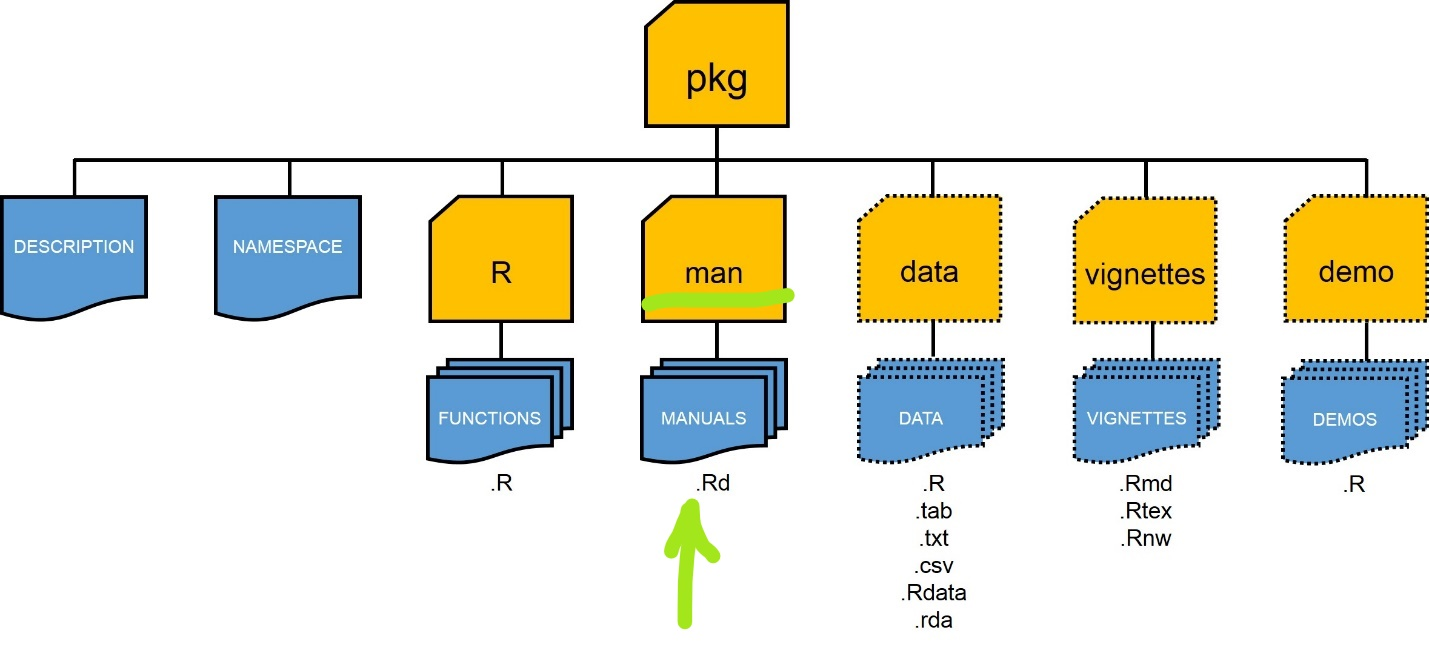
\includegraphics[width=0.9\linewidth]{Manu}
		%	\caption{}
		\label{fig:packages}
	\end{figure}
	
	
\end{frame}






\begin{frame}[t]{2.1.4 Object Documentation and Manuals}
	
	\begin{itemize}
		\item  Good Documentation	is	one	of	the	most	important	aspects	of	a	good package
		\begin{itemize}
			\item Documenting	Functions, 	Classes,	Generics and	Methods
			\item Documenting	Datasets
			\item Documenting	Packages
			\item ...
		\end{itemize}
		
		\item R	provides	a	standard	way	of	documenting	the	objects	in	a	package:	you	write	.Rd	files	in 	the	man/ directory.	
		\item 	These	files	use	a	custom	syntax,	loosely	based	on	LaTeX,	and	are
		rendered	to	HTML,	plain	text,	and	PDF	for	viewing.
		\item there are two ways to do this:
		\begin{itemize}
			\item writing	these	files	by	hand 
			\item use the package "roxygen2" (recommended)
		\end{itemize}
		
		
	\end{itemize}
	
\end{frame}











\begin{frame}[t]{2.2. Data, Vignettes, Demo}
	
	
	\begin{figure}
		\centering
		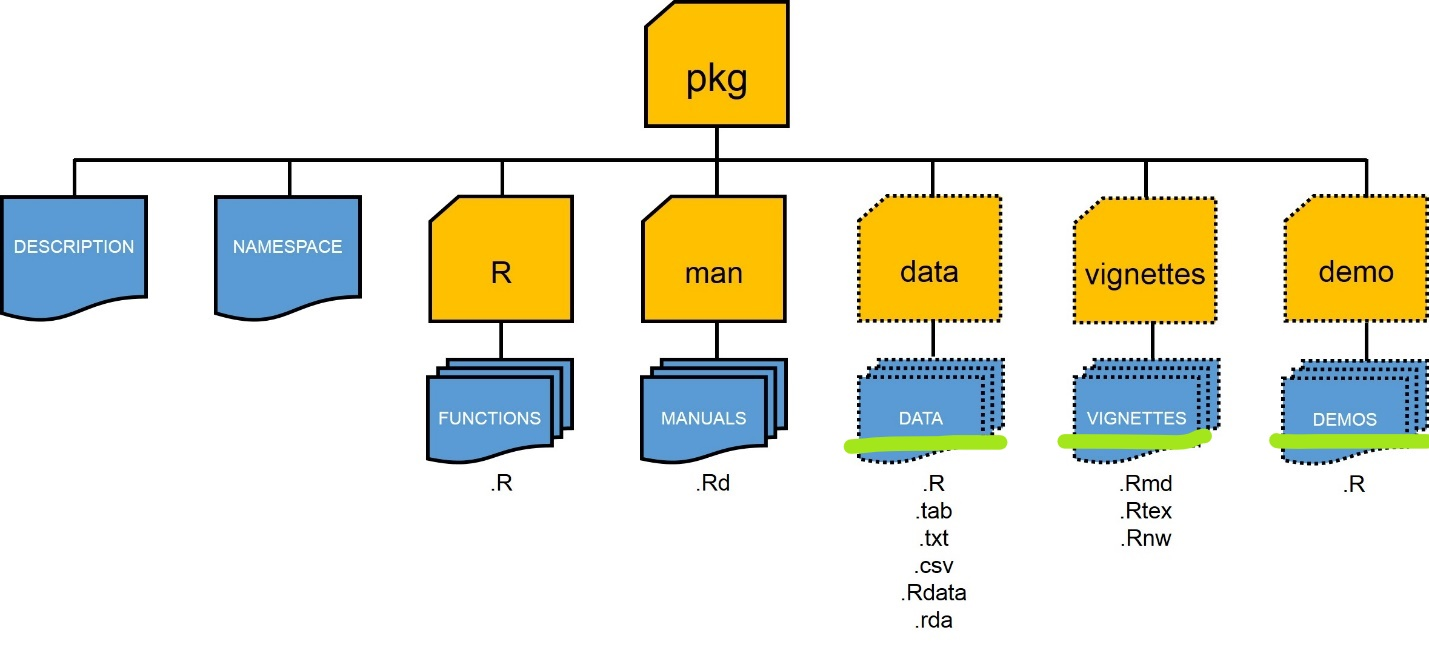
\includegraphics[width=0.9\linewidth]{opt}
		%	\caption{}
		\label{fig:packages}
	\end{figure}
	
	
\end{frame}










\begin{frame}[t]{2.2.1 Data - External Input (optional)}
	
	\begin{itemize}
		\item to	include	own data	in	a	package
		\item three	main	ways	to	include	data	in	your	package:
		\begin{itemize}
			\item store	binary	data (available for the user) in \textbf{data/}
			\item store	parsed	data (not available for the user) in
			\textbf{R/sysdata.rda}
			\item store	raw	data in	\textbf{inst/extdata}
		\end{itemize}

	\end{itemize}
	
\end{frame}






\begin{frame}[t]{2.2.2 Vignettes (optional)}
	
	\begin{itemize}
		\item  vignettes are a long-form guide to your package
		\item  describes a problem like a book	chapter	or	an	academic paper
		\item For Example: https://cran.r-project.org/web/packages/dplyr/vignettes/colwise.html
		\item The elegant way to build a vignette is to use RMarkdown and Knitr.  
		\item Workflow: 
				
		\begin{enumerate}
			\item 1.	Create	a	vignettes/	directory.
			\item Add	the	necessary	dependencies	to	DESCRIPTION
			\item Draft	a	vignette,	vignettes/my-vignette.Rmd.
		\end{enumerate}
		
	\end{itemize}
	
\end{frame}




\begin{frame}[t]{2.2.3 Demo (optional)}
	
	\begin{itemize}
		\item Demos	are	like	examples
		\item A	demo is	an .R file that	lives in \textbf{demo/}
		\item Fuseful to the introduction of vignettes
	
		
	\end{itemize}
	
\end{frame}







%%Folie_x

\begin{frame}[t]{3. Best Practices - A Quickstart Guide for own packages }
	
	\begin{block}{Das ist ein Block}
		Inhalt...
	\end{block}
	
	\begin{enumerate}
		\item hallo
		\item hallo2
	\end{enumerate}

\end{frame}









\begin{frame}[t]{xxx. Sources }
	

	
	\begin{enumerate}
		\item https://rtask.thinkr.fr/wp-content/uploads/user2019\_create\_package\_with\_pkg.png
		\item http://r-pkgs.had.co.nz/cover.png
		\item https://methodsblog.files.wordpress.com/2015/11/stott-1.jpg?w=1024\&h=464
		\item http://r-pkgs.had.co.nz/
	\end{enumerate}
	
\end{frame}


\section{Creating a Package Yourself}

\begin{frame}{Packages we will be using}

\begin{columns}

\begin{column}{0.20\textwidth}
\begin{center}

\includegraphics[width=1\textwidth]{devtools}

\end{center}
\end{column}



\begin{column}{0.20\textwidth}  
\begin{center}

\includegraphics[width=1\textwidth]{usethis} 

\end{center}
\end{column}

\begin{column}{0.20\textwidth}  
\begin{center}
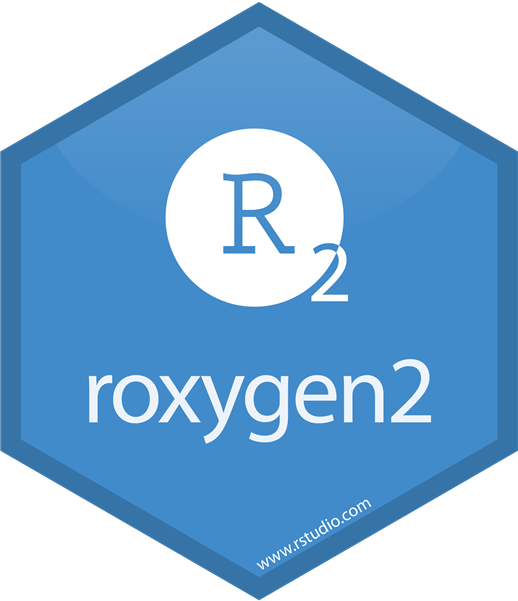
\includegraphics[width=1\textwidth]{roxygen2}
\end{center}
\end{column}
\pause
\begin{column}{0.20\textwidth}  
\begin{center}

\includegraphics[width=1\textwidth]{newnice}
\end{center}
\end{column}

\begin{column}{0.20\textwidth}  
\begin{center}

\includegraphics[width=1\textwidth]{shrek_hex}
\end{center}
\end{column}

\end{columns}

\end{frame}






\end{document}